\documentclass{beamer}

\usetheme{Warsaw}
%\usetheme{PaloAlto}
%\usetheme{CambridgeUS}
%\usetheme{Boadilla}


\usepackage{amsmath, amssymb}
\usepackage{xcolor}

\newtheorem*{conjecture}{Conjecture}

\newcommand{\Z}{\mathbb{Z}}
\newcommand{\Q}{\mathbb{Q}}
\newcommand{\C}{\mathbb{C}}
\newcommand{\R}{\mathbb{R}}
\newcommand{\N}{\mathbb{N}}
\newcommand{\F}{\mathbb{F}}
\newcommand{\Or}{\mathcal{O}}
\newcommand{\tr}{\begin{rm} tr \end{rm}}
\newcommand{\disc}{\begin{rm} disc \end{rm}}
\newcommand{\ord}{\begin{rm} ord \end{rm}}
\newcommand{\Gal}{\begin{rm} Gal \end{rm}}

\usepackage{graphicx}
\graphicspath{{/Users/Evariste/Pictures/axa_data_challenge/}}




\title{AXA Data Challenge 2016}
\subtitle{Yellow}
\author{BELLEC Maxime, HUNG Chia-Man, LIU Zhengying}
\institute{Master Data Science}
\date{January 18, 2017}

\AtBeginSection[]
{
        \begin{frame}<beamer>{Summary}
                \tableofcontents[currentsection]
        \end{frame}
}

\begin{document}


\frame{\titlepage}

\begin{frame} \frametitle{Summary}
\tableofcontents
\end{frame}


\section{Data pre-processing \& Feature engineering}

\begin{frame}
\frametitle{Data pre-processing}
\begin{itemize}
\item
Only a few columns of the training data are in test data \\

$\Rightarrow$ Keep only 3 columns:  \texttt{DATE, ASS\_ASSIGNMENT} and  \texttt{CSPL\_RECEIVED\_CALLS}

\item
Multiple columns for each \texttt{(DATE, ASS\_ASSIGNMENT)}

$\Rightarrow$ sum the \texttt{CSPL\_RECEIVED\_CALLS}
\end{itemize}
\end{frame}

\begin{frame}\frametitle{Sum the repeated rows}
\centering
\includegraphics[width=10cm]{repetition.png}

\end{frame}

\begin{frame}
\frametitle{Feature engineering}
\centering
\includegraphics[width=11cm]{feature.png}
\end{frame}



\section{Data visualization \& Preliminary analysis}

\begin{frame}\frametitle{Data visualization}
\centering
\includegraphics[width=11cm]{average.png}
\end{frame}

\begin{frame}\frametitle{Data visualization - \texttt{ASS\_ASSIGNMENT}}
\centering
\includegraphics[width=8cm]{ass.png}
\end{frame}

\begin{frame}\frametitle{Data visualization - Year}
\centering
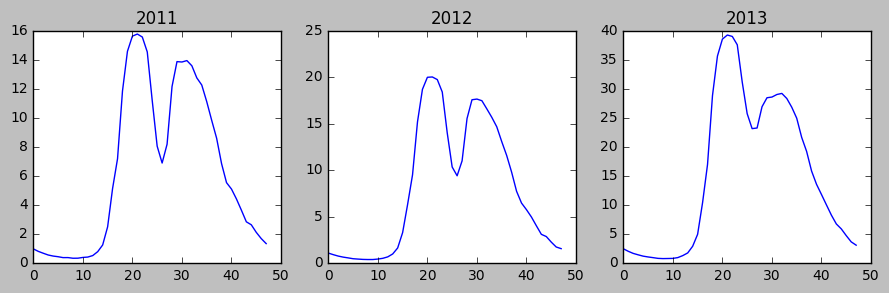
\includegraphics[width=11cm]{year.png}
\end{frame}

\begin{frame}\frametitle{Data visualization - Month}
\centering
\includegraphics[width=11cm]{month.png}
\end{frame}

\begin{frame}\frametitle{Data visualization - Weekday}
\centering
\includegraphics[width=11cm]{weekday.png}
\end{frame}

\begin{frame}\frametitle{Data visualization - \texttt{DAY\_OFF}}
\centering
\includegraphics[width=11cm]{{day_off.png}}
\end{frame}

\begin{frame}\frametitle{Data visualization - \texttt{DAY\_AFTER\_DAY\_OFF}}
\centering
\includegraphics[width=11cm]{{day_after_day_off.png}}
\end{frame}


\section{Our approaches}

\subsection{A first simple approach}

\begin{frame}\frametitle{1st approach - simple approach}
\begin{itemize}
\item
For a given \texttt{ASS\_ASSIGNMENT} and weekly time slot, such as Tuesday 09:00-09:30, the \texttt{CSPL\_RECEIVED\_CALLS} are more or less stationary
\item
The idea is to predict for each the « best stationary value » by minimizing the empirical loss
\end{itemize}
\end{frame}

\begin{frame}\frametitle{1st approach - simple approach}
The empirical loss function
$$
R(\hat{y}) = \frac{1}{n} \sum_{i=1}^n \ell(y_i,\hat{y})
$$
\pause
The best constant value
\begin{equation}
\begin{aligned}
&R'(\hat{y}) = \frac{1}{n} \sum_{i=1}^n (-\alpha e^{\alpha (y_i - \hat{y})} + \alpha) = 0 \\
\implies & \frac{1}{n} \sum_{i=1}^n  e^{\alpha (y_i - \hat{y})} = 1 \\
\implies & \hat{y} = \log \frac{1}{n} \sum_{i=1}^n  e^{\alpha y_i} = softmax(\alpha Y) - \log n
\end{aligned}
\end{equation}
\end{frame}


\begin{frame}\frametitle{1st approach - simple approach}
\begin{block}{Advantages}
\begin{itemize}
\item
Simple model
\item
Explainable
\item
Use the real loss function LinEx
\end{itemize}
\end{block}
\begin{alertblock}{Disadvantages}
\begin{itemize}
\item
Too many parameters (about 10000 lines in \texttt{predict\_table})
\item
Many of these parameters are correlated
\end{itemize}
\end{alertblock}

\begin{exampleblock}{Result}
2.55 on the leader board
\end{exampleblock}
\end{frame}


\subsection{A generalized version: Linear LinEx Regression}

\begin{frame} \frametitle{2nd approach - a generalized version}
\begin{itemize}
\item
Our 1st approach can be regarded as a \textbf{linear regression} model \\
\begin{small}
where the feature vector is “one-hot” encoding for all possible
(ASS\_ASSIGNMENT, slot, dayofweek) tuples.
\end{small}
\item
We extend it by considering more features (month, day\_off)
\item
More general: consider \textbf{all possible combinations of all
features!} \\
\pause
$\Rightarrow$ Linear LinEx Regression on Combined Features
\end{itemize}
\end{frame}


\begin{frame}[fragile] \frametitle{Combined Feature matrix}
\begin{itemize}
\item
For the row 
\begin{verbatim}
(ASS_ASSIGNMENT, dayofweek, month, slot) 
= (Crises, 5, 1, 0)
\end{verbatim}
\item
We associate a vector of 0 and 1’s, where the 1’s are in columns corresponding to
\end{itemize}
\end{frame}

\begin{frame}[fragile]\frametitle{\texttt{(ASS\_ASSIGNMENT, dayofweek, month, slot) 
= (Crises, 5, 1, 0)}}
\begin{itemize}[<+->]
\item
\begin{verbatim}
(ASS_ASSIGNMENT=Crises, dayofweek=5, month=1, slot=0)
\end{verbatim}
\item
\begin{verbatim}
(dayofweek=5, month=1, slot=0)
\end{verbatim}
\item
\begin{verbatim}
(ASS_ASSIGNMENT=Crises, month=1, slot=0)
\end{verbatim}
\item
\begin{verbatim}
(ASS_ASSIGNMENT=Crises, dayofweek=5, slot=0)
\end{verbatim}
\item
\begin{verbatim}
(ASS_ASSIGNMENT=Crises, dayofweek=5, month=1)
\end{verbatim}
\item
\begin{verbatim}
(month=1, slot=0)
\end{verbatim}
\item
\begin{verbatim}
(dayofweek=5, slot=0)
\end{verbatim}
\item
\begin{verbatim}
(dayofweek=5, month=1)
\end{verbatim}
\end{itemize}
\end{frame}

\begin{frame}[fragile]\frametitle{\texttt{(ASS\_ASSIGNMENT, dayofweek, month, slot) 
= (Crises, 5, 1, 0)}}
\begin{itemize}[<+->]
\item
\begin{verbatim}
(ASS_ASSIGNMENT=Crises, slot=0)
\end{verbatim}
\item
\begin{verbatim}
(ASS_ASSIGNMENT=Crises, month=1)
\end{verbatim}
\item
\begin{verbatim}
(ASS_ASSIGNMENT=Crises, dayofweek=5)
\end{verbatim}
\item
\begin{verbatim}
(slot=0)
\end{verbatim}
\item
\begin{verbatim}
(month=1)
\end{verbatim}
\item
\begin{verbatim}
(dayofweek=5)
\end{verbatim}
\item
\begin{verbatim}
(ASS_ASSIGNMENT=Crises)
\end{verbatim}
\item
\begin{verbatim}
()
\end{verbatim}
\pause $\Uparrow$ intercept
\end{itemize}
\end{frame}

\begin{frame}\frametitle{Combined Feature matrix}
\begin{itemize}
\item
A feature matrix of shape (1030829,147784)! 
\item
But each row has only \textbf{16 non-zero terms}
\item
$\Rightarrow$ Use \texttt{scipy.sparse.csr\_matrix}
\end{itemize}
\end{frame}

\begin{frame}\frametitle{Linear linex regression}
The loss function
$$
\frac 1n \sum_{i=1}^n \ell(y_i,x_i^\top \theta) + \frac \lambda 2 \|\theta\|_2^2
$$
where
$\ell(x,y) = LinEx(x, y) = \exp(\alpha(x - y)) - \alpha(x-y) - 1$ (LinEx regression)
\end{frame}

\begin{frame}\frametitle{Learning algorithm}
SVRG (Stochastic Variance Reduced Gradient) algorithm
\end{frame}

\begin{frame} \frametitle{SVRG algorithm}
\textbf{Input}: starting point $\theta_0$, learning rate $\eta > 0$\\
Put $\tilde{\theta}^1 \leftarrow \theta_0$ \\
For $k=1,2,...$ until convergence do
\begin{enumerate}
\item Put $\theta_0^k \leftarrow \tilde{\theta}^1_0$
\item Compute $\mu = \nabla f(\tilde{\theta}^k)$
\item For $t=0,...,m-1$:
\begin{itemize}
\item Pick uniformly at random $i$ in $\{ 1,...,n \}$
\item Apply the step
$$\theta_{t+1}^k \leftarrow \theta_t^k - \eta(\nabla f_i(\theta_t^k) - \nabla f_i(\tilde{\theta}^k)+\mu)$$
\end{itemize}
Set
$$\tilde{\theta}^k \leftarrow \frac{1}{m} \sum_{t=1}^m \theta^k_t$$
\end{enumerate}
\textbf{Return} last $\theta_t^k$
\end{frame}

\begin{frame}\frametitle{2nd approach - Linear LinEx Regression}
\begin{block}{Advantages}
\begin{itemize}
\item
The loss function is convex
\item
Very general, containing many approaches as special case
\item
Explainable
\item
Use the real loss function LinEx
\end{itemize}
\end{block}
\begin{alertblock}{Disadvantages}
\begin{itemize}
\item
Many parameters (about 150000 of them)
\item
Hard to optimize
\end{itemize}
\end{alertblock}

\begin{exampleblock}{Result}
1.99 on the leader board
\end{exampleblock}
\end{frame}

\subsection{Random Forest}

\begin{frame}\frametitle{3rd approach - Random Forest}
\begin{itemize}
\item
Use all the features in feature engineering
\item
No categorical values in sklearn $\Rightarrow$ one-hot encoding
\item
Remove Evenements and Gestion Amex
\item
Cross validation (80\% training, 20\% testing)
\item
Multiply by C = 2.4
\end{itemize}•
\end{frame}

\begin{frame}\frametitle{3rd approach - Random Forest}
\begin{block}{Advantages}
\begin{itemize}
\item
Robust model
\item
Existing library
\item
Relatively good results
\end{itemize}
\end{block}
\begin{alertblock}{Disadvantages}
\begin{itemize}
\item
Parameter tuning
\item
Hard to use a custom loss function
\end{itemize}
\end{alertblock}
\begin{exampleblock}{Result}
1.175 on the leaderboard
\end{exampleblock}
\end{frame}

\section{Conclusion}

\begin{frame}\frametitle{Conclusion}
\begin{itemize}
\item
For prediction, when collecting data on past time, make sure this data will also be available for future times, otherwise they are not useful features for prediction
\item
A lot of features can be created on DATE and it can be enough when the data actually mostly depends on DATE
\end{itemize}
\end{frame}













\end{document}